\begin{exercice}
    \begin{minipage}{0.5\linewidth}
        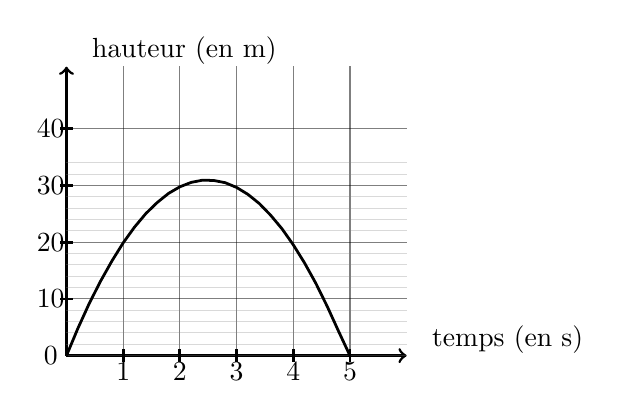
\begin{tikzpicture}[baseline,scale=0.4]
            \tikzset{
                point/.style={
                    thick,
                    draw,
                    cross out,
                    inner sep=0pt,
                    minimum width=5pt,
                    minimum height=5pt,
                },
            }
            \draw[color ={black},line width = 1,->] (0,0)--(10.8,0);
            \draw[color ={black},line width = 1,->] (0,0)--(0,9.175571413994916);
            \draw[color ={black},opacity = 0.5] (0,1.8)--(10.8,1.8);
            \draw[color ={black},opacity = 0.5] (0,3.6)--(10.8,3.6);
            \draw[color ={black},opacity = 0.5] (0,5.4)--(10.8,5.4);
            \draw[color ={black},opacity = 0.5] (0,7.2)--(10.8,7.2);
            \draw[color ={black},opacity = 0.5] (1.8,0)--(1.8,9.18);
            \draw[color ={black},opacity = 0.5] (3.6,0)--(3.6,9.18);
            \draw[color ={black},opacity = 0.5] (5.4,0)--(5.4,9.18);
            \draw[color ={black},opacity = 0.5] (7.2,0)--(7.2,9.18);
            \draw[color ={black},opacity = 0.5] (9,0)--(9,9.18);
            \draw[color ={gray},opacity = 0.3] (0,0)--(10.8,0);
            \draw[color ={gray},opacity = 0.3] (0,0.36)--(10.8,0.36);
            \draw[color ={gray},opacity = 0.3] (0,0.72)--(10.8,0.72);
            \draw[color ={gray},opacity = 0.3] (0,1.08)--(10.8,1.08);
            \draw[color ={gray},opacity = 0.3] (0,1.44)--(10.8,1.44);
            \draw[color ={gray},opacity = 0.3] (0,2.16)--(10.8,2.16);
            \draw[color ={gray},opacity = 0.3] (0,2.52)--(10.8,2.52);
            \draw[color ={gray},opacity = 0.3] (0,2.88)--(10.8,2.88);
            \draw[color ={gray},opacity = 0.3] (0,3.24)--(10.8,3.24);
            \draw[color ={gray},opacity = 0.3] (0,3.96)--(10.8,3.96);
            \draw[color ={gray},opacity = 0.3] (0,4.32)--(10.8,4.32);
            \draw[color ={gray},opacity = 0.3] (0,4.68)--(10.8,4.68);
            \draw[color ={gray},opacity = 0.3] (0,5.04)--(10.8,5.04);
            \draw[color ={gray},opacity = 0.3] (0,5.76)--(10.8,5.76);
            \draw[color ={gray},opacity = 0.3] (0,6.12)--(10.8,6.12);
            \draw[color ={black},line width = 1] (1.8,-0.2)--(1.8,0.2);
            \draw[color ={black},line width = 1] (3.6,-0.2)--(3.6,0.2);
            \draw[color ={black},line width = 1] (5.4,-0.2)--(5.4,0.2);
            \draw[color ={black},line width = 1] (7.2,-0.2)--(7.2,0.2);
            \draw[color ={black},line width = 1] (9,-0.2)--(9,0.2);
            \draw[color ={black},line width = 1] (-0.2,1.8)--(0.2,1.8);
            \draw[color ={black},line width = 1] (-0.2,3.6)--(0.2,3.6);
            \draw[color ={black},line width = 1] (-0.2,5.4)--(0.2,5.4);
            \draw[color ={black},line width = 1] (-0.2,7.2)--(0.2,7.2);
            \draw [color={black},fill opacity = 1] (1.8,-0.5) node[anchor = center,scale=1] {$1$};
            \draw [color={black},fill opacity = 1] (3.6,-0.5) node[anchor = center,scale=1] {$2$};
            \draw [color={black},fill opacity = 1] (5.4,-0.5) node[anchor = center,scale=1] {$3$};
            \draw [color={black},fill opacity = 1] (7.2,-0.5) node[anchor = center,scale=1] {$4$};
            \draw [color={black},fill opacity = 1] (9,-0.5) node[anchor = center,scale=1] {$5$};
            \draw [color={black},fill opacity = 1] (-0.5,1.8) node[anchor = center,scale=1] {$10$};
            \draw [color={black},fill opacity = 1] (-0.5,3.6) node[anchor = center,scale=1] {$20$};
            \draw [color={black},fill opacity = 1] (-0.5,5.4) node[anchor = center,scale=1] {$30$};
            \draw [color={black},fill opacity = 1] (-0.5,7.2) node[anchor = center,scale=1] {$40$};
            \draw [color={black},fill opacity = 1] (11.3,0.5) node[anchor = west,scale=1] {temps (en s)};
            \draw [color={black},fill opacity = 1] (0.5,9.68) node[anchor = west,scale=1] {hauteur (en m)};            
            \draw[color={black},line width = 1] (0,0)--(0.36,0.86)--(0.72,1.65)--(1.08,2.36)--(1.44,3)--(1.8,3.58)--(2.16,4.08)--(2.52,4.51)--(2.88,4.86)--(3.24,5.15)--(3.6,5.36)--(3.96,5.5)--(4.32,5.57)--(4.68,5.56)--(5.04,5.49)--(5.4,5.34)--(5.76,5.12)--(6.12,4.83)--(6.48,4.46)--(6.84,4.03)--(7.2,3.52)--(7.56,2.94)--(7.92,2.29)--(8.28,1.56)--(8.64,0.77)--(9,0);
            \draw [color={black},fill opacity = 1] (-0.5,0) node[anchor = center,scale=1] {$0$};
        \end{tikzpicture}
    \end{minipage}
    \begin{minipage}{0.43\linewidth}
        On a représenté l'évolution de la hauteur d'un projectile lancé depuis le sol (en m) en fonction du temps (en secondes).    
        \begin{enumerate}
            \item Déterminer au bout de combien de temps le projectile retombe au sol.
            \item Déterminer la hauteur maximale atteinte par le projectile.
        \end{enumerate}
    \end{minipage}
\end{exercice}
\begin{corrige}
    \phantom{rrr}

    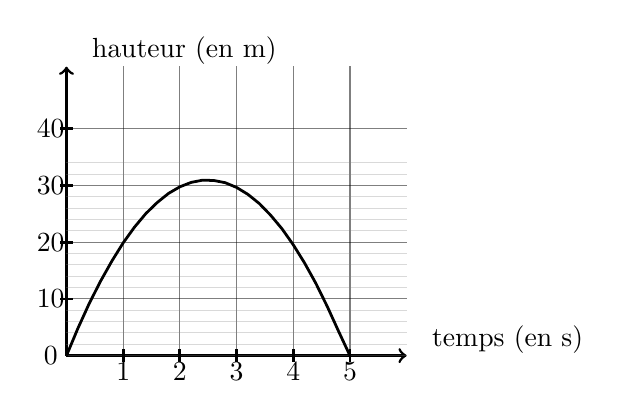
\begin{tikzpicture}[baseline,scale=0.4]
        \tikzset{
            point/.style={
                thick,
                draw,
                cross out,
                inner sep=0pt,
                minimum width=5pt,
                minimum height=5pt,
            },
        }
        \draw[color ={black},line width = 1,->] (0,0)--(10.8,0);
        \draw[color ={black},line width = 1,->] (0,0)--(0,9.175571413994916);
        \draw[color ={black},opacity = 0.5] (0,1.8)--(10.8,1.8);
        \draw[color ={black},opacity = 0.5] (0,3.6)--(10.8,3.6);
        \draw[color ={black},opacity = 0.5] (0,5.4)--(10.8,5.4);
        \draw[color ={black},opacity = 0.5] (0,7.2)--(10.8,7.2);
        \draw[color ={black},opacity = 0.5] (1.8,0)--(1.8,9.18);
        \draw[color ={black},opacity = 0.5] (3.6,0)--(3.6,9.18);
        \draw[color ={black},opacity = 0.5] (5.4,0)--(5.4,9.18);
        \draw[color ={black},opacity = 0.5] (7.2,0)--(7.2,9.18);
        \draw[color ={black},opacity = 0.5] (9,0)--(9,9.18);
        \draw[color ={gray},opacity = 0.3] (0,0)--(10.8,0);
        \draw[color ={gray},opacity = 0.3] (0,0.36)--(10.8,0.36);
        \draw[color ={gray},opacity = 0.3] (0,0.72)--(10.8,0.72);
        \draw[color ={gray},opacity = 0.3] (0,1.08)--(10.8,1.08);
        \draw[color ={gray},opacity = 0.3] (0,1.44)--(10.8,1.44);
        \draw[color ={gray},opacity = 0.3] (0,2.16)--(10.8,2.16);
        \draw[color ={gray},opacity = 0.3] (0,2.52)--(10.8,2.52);
        \draw[color ={gray},opacity = 0.3] (0,2.88)--(10.8,2.88);
        \draw[color ={gray},opacity = 0.3] (0,3.24)--(10.8,3.24);
        \draw[color ={gray},opacity = 0.3] (0,3.96)--(10.8,3.96);
        \draw[color ={gray},opacity = 0.3] (0,4.32)--(10.8,4.32);
        \draw[color ={gray},opacity = 0.3] (0,4.68)--(10.8,4.68);
        \draw[color ={gray},opacity = 0.3] (0,5.04)--(10.8,5.04);
        \draw[color ={gray},opacity = 0.3] (0,5.76)--(10.8,5.76);
        \draw[color ={gray},opacity = 0.3] (0,6.12)--(10.8,6.12);
        \draw[color ={black},line width = 1] (1.8,-0.2)--(1.8,0.2);
        \draw[color ={black},line width = 1] (3.6,-0.2)--(3.6,0.2);
        \draw[color ={black},line width = 1] (5.4,-0.2)--(5.4,0.2);
        \draw[color ={black},line width = 1] (7.2,-0.2)--(7.2,0.2);
        \draw[color ={black},line width = 1] (9,-0.2)--(9,0.2);
        \draw[color ={black},line width = 1] (-0.2,1.8)--(0.2,1.8);
        \draw[color ={black},line width = 1] (-0.2,3.6)--(0.2,3.6);
        \draw[color ={black},line width = 1] (-0.2,5.4)--(0.2,5.4);
        \draw[color ={black},line width = 1] (-0.2,7.2)--(0.2,7.2);
        \draw [color={black},fill opacity = 1] (1.8,-0.5) node[anchor = center,scale=1] {$1$};
        \draw [color={black},fill opacity = 1] (3.6,-0.5) node[anchor = center,scale=1] {$2$};
        \draw [color={black},fill opacity = 1] (5.4,-0.5) node[anchor = center,scale=1] {$3$};
        \draw [color={black},fill opacity = 1] (7.2,-0.5) node[anchor = center,scale=1] {$4$};
        \draw [color={black},fill opacity = 1] (9,-0.5) node[anchor = center,scale=1] {$5$};
        \draw [color={black},fill opacity = 1] (-0.5,1.8) node[anchor = center,scale=1] {$10$};
        \draw [color={black},fill opacity = 1] (-0.5,3.6) node[anchor = center,scale=1] {$20$};
        \draw [color={black},fill opacity = 1] (-0.5,5.4) node[anchor = center,scale=1] {$30$};
        \draw [color={black},fill opacity = 1] (-0.5,7.2) node[anchor = center,scale=1] {$40$};
        \draw [color={black},fill opacity = 1] (11.3,0.5) node[anchor = west,scale=1] {temps (en s)};
        \draw [color={black},fill opacity = 1] (0.5,9.68) node[anchor = west,scale=1] {hauteur (en m)};            
        \draw[color={black},line width = 1] (0,0)--(0.36,0.86)--(0.72,1.65)--(1.08,2.36)--(1.44,3)--(1.8,3.58)--(2.16,4.08)--(2.52,4.51)--(2.88,4.86)--(3.24,5.15)--(3.6,5.36)--(3.96,5.5)--(4.32,5.57)--(4.68,5.56)--(5.04,5.49)--(5.4,5.34)--(5.76,5.12)--(6.12,4.83)--(6.48,4.46)--(6.84,4.03)--(7.2,3.52)--(7.56,2.94)--(7.92,2.29)--(8.28,1.56)--(8.64,0.77)--(9,0);
        \draw [color={black},fill opacity = 1] (-0.5,0) node[anchor = center,scale=1] {$0$};
    \end{tikzpicture}

        On a représenté, l'évolution de la hauteur d'un projectile lancé depuis le sol (en m) en fonction du temps (en secondes).    
        
        \begin{enumerate}
            \item Déterminer au bout de combien de temps le projectile retombe au sol.
            
            {\red Le projectile retombe au sol au bout de 5s.}
            \item Déterminer la hauteur maximale atteinte par le projectile.
            
            {\red La hauteur maximale atteinte par le projectile vaut environ \Lg[m]{31}, au bout de \num{2.5}s.}
        \end{enumerate}
\end{corrige}